\subsection*{Teil B: Geometrische Berechnungen (25 Minuten)}

\begin{enumerate}[resume, label=\arabic*.]
    \item \textbf{Rechteck:} Länge = 8 cm, Breite = 5 cm

    \begin{enumerate}[label=\alph*)]
        \item Umfang: $U = 2 \cdot (l + b) = 2 \cdot (8 + 5)$ cm = \underline{\hspace{3cm}}
        \item Flächeninhalt: $A = l \cdot b = 8 \cdot 5$ cm² = \underline{\hspace{3cm}}
    \end{enumerate}

    \vspace{0.5cm}

    \item \textbf{Dreieck:} Grundseite $g = 6$ cm, Höhe $h = 4$ cm

    Flächeninhalt: $A = \dfrac{g \cdot h}{2} = \dfrac{6 \cdot 4}{2}$ cm² = \underline{\hspace{3cm}}

    \vspace{0.5cm}

    \item \textbf{Quader:} Länge = 4 cm, Breite = 3 cm, Höhe = 5 cm

    \begin{enumerate}[label=\alph*)]
        \item Volumen: $V = l \cdot b \cdot h = 4 \cdot 3 \cdot 5$ cm³ = \underline{\hspace{3cm}}

        \item Oberfläche: 
        \begin{align*}
            O &= 2 \cdot (l \cdot b + l \cdot h + b \cdot h)\\
            &= 2 \cdot (4 \cdot 3 + 4 \cdot 5 + 3 \cdot 5) \text{ cm}^2\\
            &= 2 \cdot (\underline{\hspace{1cm}} + \underline{\hspace{1cm}} + \underline{\hspace{1cm}}) \text{ cm}^2\\
            &= 2 \cdot \underline{\hspace{2cm}} \text{ cm}^2 = \underline{\hspace{3cm}}
        \end{align*}
    \end{enumerate}

    \vspace{0.5cm}

    \item \textbf{Koordinaten:}

    Zeichne das Viereck mit den Eckpunkten $A(1\|1), B(4|1), C(4|3), D(1|3)$

    \begin{center}
        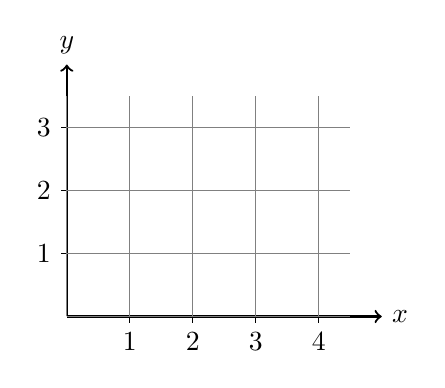
\begin{tikzpicture}[scale=0.8]
            \draw[thick,->] (0,0) -- (5,0) node[right] {$x$};
            \draw[thick,->] (0,0) -- (0,4) node[above] {$y$};
            \foreach \x in {1,2,3,4}
            \draw (\x,0.1) -- (\x,-0.1) node[below] {\x};
            \foreach \y in {1,2,3}
            \draw (0.1,\y) -- (-0.1,\y) node[left] {\y};
            \draw[thin,gray,step=1] (0,0) grid (4.5,3.5);
        \end{tikzpicture}
    \end{center}

    \begin{itemize}
        \item Was für ein Viereck ist es? \underline{\hspace{4cm}}
        \item Berechne seinen Flächeninhalt: $A = $ \underline{\hspace{4cm}}
    \end{itemize}
\end{enumerate}